\documentclass{llncs}
%
\usepackage{amsmath}
\usepackage{amsfonts}
\usepackage{pgfplots}
\usepackage{graphicx}
%
          \clubpenalty = 10000
          \widowpenalty = 10000
          \displaywidowpenalty = 10000

\pgfplotsset{compat=1.17} 
\begin{document}
%
%
\title{Lesser Evil: Embracing Failure to Protect Overall System Availability}
%
\titlerunning{Lesser Evil}
%
\author{Vikt\'oria F{\"o}rd\H{o}s\inst{1,2}\orcidID{0000-0001-6403-9797} \and \\
Alexandre Jorge Barbosa Rodrigues\inst{1}\orcidID{0000-0001-7618-6743}}
%
\authorrunning{V. F{\"o}rd\H{o}s \and A. J. Barbosa Rodrigues}
% 
\institute{Cisco Systems, Stockholm, Sweden \and
ELTE, E{\"o}tv{\"o}s Lor\'and University, Faculty of Informatics, Budapest, Hungary
\email{\{vfordos,albarbos\}@cisco.com}}
%
\maketitle              % typeset the header of the contribution
%

\begin{abstract}
Low memory conditions degrade system performance, challenge programs to fulfil their SLA and can lead to out-of-memory errors causing a major system outage. Running low on memory is an especially dangerous  situation in case of mission critical, embedded Erlang systems with high availability requirements. In such systems, total system outage must be avoided at all costs. Nonetheless, no solution exists today that can be added to an Erlang system without code modification and would treat memory pressure out of the box.

We propose an approach, called Lesser Evil, that can treat low memory pressure in any fault-tolerant Erlang system without the need of any code modification. Our experiments suggest that, with the help of Lesser Evil, an embedded Erlang system can survive low memory conditions and avoid a major outage.
\end{abstract}
%

\keywords{Embedded systems, Memory management, Fault tolerance, Erlang.}

\section{Introduction}
In our digitalised world we depend on mission critical, embedded systems.  These systems need to be always available  regardless of the current load on the system. Parallelism is a key enabler to accommodate a system to variable workload. However, what stays constant in a system is the total memory installed (per a single host). If a system runs low on available memory, it will not perform as expected. Since it is struggling to allocate memory enough to execute requests, it will not satisfy its QoS metrics, neither SLA requirements. Considering best case scenarios, its performance will degrade while in the worst case the program will stop with an out-of-memory error causing the system to reboot. Taking into account that embedded systems have strongly constrained resources and slow processing capabilities, the reboot can take significant amount of time while the system stays offline. Hence, running low on memory is a critical event in case of mission critical, embedded systems that should not be ignored as it can compromise the availability of the system.

The presented problem is especially relevant in case of embedded systems that are written in Erlang. The Erlang programming language was designed in the Ericsson software technology lab for systems that will never stop or fail. Early use cases of Erlang at Ericsson include a multi-service switch, AXD 301~\cite{axd}, where the control system was implemented in Erlang. Since then, Erlang has become well-known and used in the telecommunication segment, multiple companies have decided to adapt Erlang to implement mission critical, embedded systems. An illustrative example of the significance of Erlang in this sector is that Cisco ships about 2 million devices per year with Erlang in them and that 90\% of all internet traffic goes through Erlang controlled nodes~\cite{johan}.

%Treating memory pressure on a single host is a well-known challenge, multiple solutions have been proposed. Solutions range from operating system level~\cite{embracingfailures,oom} to the usage of programming models with specific runtime systems~\cite{itasks}. The problem with operating system level solutions is that they are not fine grained enough, as they aim to protect the overall host. The result can be catastrophic: the most important program can be their victim. Solutions on the other end of the spectrum are application specific and have the tendency to require the adaptation of programming models and the usage of special libraries. If these requirements were not taken into account at the design phase, adding these solutions can require major redesign and rewrite of the code.
 
\emph{Motivation.} Running low on memory is an especially dangerous  situation in case of mission critical, real-time embedded systems with high availability requirements. In such systems, total system outage must be avoided at all cost, even by allowing temporary, partial failures. Nonetheless, no solution exists today that can be added to an Erlang system without code modification and would treat memory pressure out of the box. Having such a solution would enable existing Erlang systems to perform better under low memory conditions. It would help any Erlang system to deal with unexpectedly large workload  but \emph{would be very beneficial for embedded systems} where virtual memory is disabled and physical memory is very limited and constrained. %The solution should be fine grained enough to understand, pinpoint and heal the components of the software that are responsible for the most memory usage without damaging the overall system. There is a need to understand what requirements a programming language and runtime system should satisfy to enable such solution: how can memory be freed in a way that will not compromise the system, what strategies to use to select the components most responsible for the memory pressure and what compensating actions are available.

\emph{Our contributions.} %In this paper we show what requirements a programming language and the runtime system should meet in order to manage memory pressure on a single host. 
In this paper, we propose an approach, called Lesser Evil, that can treat memory pressure in any Erlang system without the need of any code modification. Lesser Evil is ready to use and is applicable to any fault-tolerant Erlang systems. We discuss why our approach is viable, how it identifies low memory conditions, what strategy it employs and how it treats memory pressure.

\emph{Summary of results.} Our evaluation shows that an Erlang system can survive and keep functioning under low memory conditions with the help of our approach. We have confirmed that Lesser Evil's strategy is correct: it is able to identify and execute compensating actions on the components most responsible for the situation without damaging the other components or the overall system.

\section{Problem Statement}

Let us take an imaginary, fault-tolerant, embedded Erlang system as a motivating example. The Erlang system is designed to run on and control an embedded device with limited memory and slow processing capability. The Erlang system and the device are expected to be always available. The Erlang system receives administrative requests that it processes, and as a result of processing, it executes commands on the embedded device. The Erlang system usually receives a few, small requests that never fills up the device memory, but sometimes a large request arrives that may require all the available memory of the device to process. If part of the device memory is used to process other small requests, the available memory is not enough to process the large requests: the device runs out of memory, becomes unresponsive or it even reboots.

To protect the availability of the device, the only available solution to use today is a generic solution for Linux systems, called the Out of Memory Manager (OOM manager)~\cite{oom}. However, the OOM manager is not an option in our example, as the OOM manager would terminate the whole Erlang system that controls the device; making the device unavailable. A more fine grained solution would be more appreciated that would not cause the termination of the whole Erlang system. Instead, it would free up enough memory to resume the normal operation of the Erlang system, for example, by terminating the large request.

The motivating example illustrates that we need a solution that treats memory pressure differently. The primary goal is to free up enough memory to resume the normal operation of the Erlang system. When releasing memory we accept local failures but we cannot tolerate abnormal termination of the whole Erlang system neither the risk of introducing permanent data inconsistencies. Under local failures we mean failures that may effect some end-user but not all users and also failures that may result in interruption of some requests but not all requests. Our goal is to prevent a major outage, but we accept temporary, partial system degradations.

To achieve our goals, a tool is needed that is able to monitor, assess and interact with the running Erlang system. The tool needs to monitor the running Erlang system to identify low memory conditions. If low memory conditions are identified the tool needs to select some entities to execute compensating actions. The tool needs to have a strategy to select entities and the strategy should consider multiple criteria when making the selection. The strategy should be based on metrics of the entities gathered from the runtime, and characterise the \emph{badness} of the entity. Compensating actions need to be defined on entity level, ensuring that the impact of the action is limited; will not have a negative impact on the overall Erlang system.
%
%\section{Treating Memory Pressure}
%In this section we briefly outline the fundamental ideas regarding our approach and we show the requirements our approach puts on programming languages and runtime systems. 
%
%\subsection{The Idea}
%
%The primary goal is to free up enough memory to resume the normal operation of the program. When releasing memory we accept local failures but we cannot tolerate abnormal termination of the program neither the risk of introducing permanent data inconsistencies. Under local failures we mean failures that may effect some end-user but not all users and also failures that may result in interruption of some requests but not all requests. Our goal is to prevent a major outage, but we accept temporary, partial system degradations.
%
%To achieve our goals, a tool is needed that is able to monitor, assess and interact with the running program. The tool needs to monitor the running program to identify low memory conditions. If low memory conditions are identified the tool needs to select some entities to execute compensating actions. The tool needs to have a strategy to select entities and the strategy should consider multiple criteria when making the selection. The strategy should be based on metrics of the entities gathered from the runtime, and characterise the \emph{badness} of the entity. Compensating actions need to be defined on entity level, ensuring that the impact of the action is limited; will not have a negative impact on the overall program.
%
%\subsection{Requirements on Programming Languages and Runtime Systems}
%In this section we discuss what is required from a programming language and its runtime system to enable out-of-the-box memory pressure management on a single host. 
%
%\emph{Entities in the Runtime System}
%The first question we should discuss is what entities the tool should work with. The decision should be based on what entity holds memory in the program. Are those OS threads, OS processes, or lightweight processes that exist only in the runtime system? These entities need to be monitored on runtime system level in order to identify their current memory allocations. Hence, the runtime system needs to provide ready-to-use metrics or routines to gather this information.
%
%\emph{Characteristics of the Entities}
%A good strategy of selecting building blocks should take into account more information than the amount of allocated memory. %It should limit the side effect of executing the compensating action on the program 
%
%First of all, in a parallel program, not all entities are equally important. Consider the difference between a process responsible for handling the write-ahead log of a database system and a process handling a single user request. The former is critical to the system and should be protected while the latter can be terminated to relax memory pressure. Another perspective to criticality is how central the entity is. The more central the entity is, the more entities depend on it, hence the more protection it needs to avoid total program failure. Identifying and listing the critical entities can only be done by the programmer, but the list needs to be fixed and independent from the current runtime status of the program. Besides, the listed entities need to be locatable by the runtime system.
%
%Second, as any parallel program includes some level of synchronisation, coordination and communication among its entities, identifying these interactions is crucial to limit the effect of compensating actions. The strategy of selecting entities needs to take this information into account, that the runtime system should provide.
%
%Third, the strategy should maximise the impact of the compensating action by selecting entities with bad future outlook. An entity has bad future outlook if we cannot expect it will release memory any time soon. A way to measure this is by looking at the amount of work it still needs to complete before it terminates. Therefore, the runtime system needs to provide a way to determine this information.
%
%Last but not least, the strategy needs to understand the effect of freeing up memory of an entity from other entities' perspective. Freeing up memory referenced by other entities would cause runtime errors. The runtime system needs to guide the strategy in this matter.
%
%\emph{Interacting with the Entities}
%When the strategy has selected the entities we know what entities are the most responsible for the memory pressure. The next question is what compensating actions are possible. This is determined by on what level the runtime system supports interacting with the entities. Does the runtime system allow us to trigger garbage collection only on a single entity, or does it allow us to de-schedule and terminate the entity and then free up its memory? How will this effect the overall program?
%
%%\subsection{Feasibility of Requirements}
%%In this section we summarise how feasible the requirements are for the programming languages we have studied. We summarise our learnings regarding Java and C\#. We have selected these two programming languages as they are managed languages, designed for and heavily used in production.
%%
%%%Considering the C programming language, interaction with a running program is very limited. One would need to implement the tool as a library and include it in the executable. This constraint defies the requirement that the tool should work out of the box and should not require any source code modification.
%%
%%Considering the Java and the C\# ecosystems, interaction with the running program is possible through the runtime system. As for entities we could choose threads, as they hold memory. The compensating action could be to terminate the thread. However, there are multiple problems with this approach. First, terminating the thread may not trigger immediate garbage collection. Second, shared resources owned by the thread will be destroyed as well, causing runtime program errors in other threads using the shared resource.  Third, unexpected termination of threads are considered runtime errors. In summary, the major obstacles arise from the usage of shared resources and the fact that threads are not allowed to fail.
%
%\emph{Summary}
%Observe that the requirements are satisfied by languages that allow runtime interaction, the entities share a very little resources, and the entities are allowed to fail. The Erlang ecosystem is a good example, it is a perfect candidate for our approach.
%


\section{Erlang}
\label{sec:erlang}
In this section we discuss the Erlang ecosystem and highlight its key features that our approach uses to treat memory pressure. 

Erlang~\cite{erlang} is a dynamically typed functional programming language that has built-in support for concurrency and distribution. Erlang systems are well known about their high availability, thanks to their failure handling and hot code loading capabilities.

An Erlang system can be considered as an actor based system, built up of interacting Erlang processes. Erlang processes~\cite{processes} are light-weight processes with small memory overhead, fast to create and terminate, and the scheduling overhead is low. The Erlang processes communicate with each other via asynchronous message passings~\cite{message-passing}. They share nothing with the outside world, they exclusively own their data (excl. large binaries that are reference counted and stored in a shared heap). If data is shared between two processes (via message passing), the data is copied to the another process's heap. Processes, while scheduled, are executing code, which is measured in \emph{reductions}. The scheduler~\cite{scheduler} de-schedules a process after a certain amount of reductions or when the process enters into a waiting state (e.g. waiting for messages or IO). The fact that processes share nothing and that they can yield to be de-scheduled enables Erlang's garbage collector~\cite{garbage-collector} to work on a single process at a time without interfering with other running processes. Moreover, when an Erlang process terminates all its allocated memory can be freed as there are no other users to those memory blocks. 

Fault tolerance is built into the language~\cite{fault-tolerance}, processes are allowed to fail. Hence, interacting processes can never assume that their peer is alive. To detect the termination of their peer, processes can monitor other processes. If the monitored process terminates, the process will be notified by a message. If the interacting processes depend on each other they can use another language construct, called the process link. A process link is a bidirectional link forwarding  events of termination, called error signals, between the linked processes. The forwarded error signal may terminate the receiving process as well, depending whether the process trapping exits. Using links and monitors more complex and robust architectures can be built that define restart strategies for the important processes. An example is the supervisor process~\cite{supervisor} that is responsible for starting, terminating and restarting its children. A common practice is to build supervisor trees that allow managing processes in a structured way and handling runtime errors where it is convenient. 

From the system architecture point of view, an Erlang system is built up from a single or a set of Erlang nodes organised into a full mesh cluster.  An Erlang node, which is an OS process, is built up from the Erlang Runtime System (ERTS) and the Erlang release. An Erlang release~\cite{release} consists of a set of Erlang applications. The Erlang applications~\cite{application} are the reusable units of the Erlang ecosystem, can be bundled into multiple releases  and be part of different deployments. (Readers experienced in the Java programming language can consider Erlang applications as Java packages.) An Erlang application is the implementation of a functionality and can cooperate with other Erlang applications to implement more complex functionality. An Erlang application defines and includes its Erlang processes. When an application starts the runtime starts an application\_master process as the main responsible process for the application. The application\_master in turn starts a process called 'x' that is responsible for the IO and to start the main supervisor for the application. The main supervisor is the first processes implemented by the user, the root of the supervisor tree for the application. The ERTS enables interaction with the running Erlang node. Processes can be created and terminated, and existing processes can be inspected at runtime: various process metrics can be retrieved. Applications can be started, stopped and upgraded without stopping the Erlang node.

%To conclude, the share nothing concept, the fault tolerance properties and the interaction opportunities of Erlang make Erlang an ideal candidate for our approach.

\section{Lesser Evil}
In this section we describe our approach  for Erlang systems, called Lesser Evil~\cite{lesser-evil}.
%\footnote{Note to reviewers: We will open source the applications once the paper has been accepted. The code is available for review upon request} 
First, we outline the approach and then we discuss the details: what entities are considered, how badness is characterised, how the strategy is evaluated and what compensating actions are employed. We show the architecture and discuss the different ways the approach can be added to an Erlang system.

Our approach aims at treating memory pressure of an Erlang system without the need of code modification. It proposes to monitor the running program and upon low memory conditions select some entities with the greatest  badness values and execute compensating actions on the selected entities. Mapping the approach to Erlang systems, the approach monitors an Erlang node and collect its memory consumption. As Erlang processes are owning their data, they hold memory in the system, thus the Erlang processes are the entities. The goal is to characterise the badness of processes with the help of process level metrics. As the runtime provides interaction possibilities with the running system, the approach employs two compensating actions: triggering garbage collection on a selected process, and terminating the process.

\subsection{Entities}
\label{sec:entities}

Lesser Evil considers Erlang processes as entities. However, it does not consider all processes, as there are critical processes in an Erlang node. As examples, consider the various system processes started by the runtime and the processes belonging to critical user applications. Automatically identifying and excluding the system processes is possible, however, distinguishing between critical and non-critical user processes is not. Lesser Evil takes the approach of letting the user decide, and requires a list of Erlang applications that are non-critical for the system (e.g. the implementation of an HTTP API). Processes belonging to the listed applications are considered only. However, this is still not enough. As discussed in Section~\ref{sec:erlang}, each application includes 3 critical processes (application\_master, process 'x' and the main supervisor of the application) that must be excluded. If they terminate, the whole application terminates, which must be prevented. 

\subsection{Badness}
\label{sec:badness}

Determining the badness of processes is the heart of the strategy: the compensating actions executed on the selected processes should help the Erlang node to survive low memory conditions, and their negative impact on the rest of the processes should be minimal.  In this section we discuss how such a metric can be constructed.

To treat memory pressure effectively, the badness assigns greater values to processes that (1) have high memory usage; (2) have several pending tasks, therefore, they have a bad future outlook.

To minimise the negative impact of the compensating actions on the rest of the processes, the badness assigns lower values to processes that (1) are long-lived and, therefore, have proven their good behaviour; (2) are important to the user; (3) play a central role in the system in the sense of several processes depend on them.

In conclusion, the goal is to select isolated, relatively new processes with high memory usage and a bad future outlook. Therefore, the $\mathit{badness}$ is a composite metric that assigns a real value to a process based on the following process level metrics.
\begin{itemize}
\item $\mathit{Memory}$. Number of bytes the process uses.
\item $\mathit{MessageQLength}$. Number of messages delivered to but not yet processed by the process. The metric expresses how much more tasks a process has pending.
\item $\mathit{Reds}$. Reduction count shows the amount of work the process has done. As for long lived processes this value can be several order of magnitudes large, the logarithm with base $10$ is applied to the reduction count in the badness formula.
\item $\mathit{Age}$. Number of checks the process has stayed alive. 
\item $\mathit{Links}$. The number of processes linking to the process. The metric expresses how central the process is.
\item $\mathit{Mons}$. The number of processes monitoring the process. The metric expresses how central the process is.
\item $\mathit{Prio}$. Erlang processes can have different priorities. The higher the process priority is, the more important the process to the user is. This is what the metric expresses by selecting a value from $\{1,10,100\}$.
\end{itemize}
The $\mathit{badness}$ metric that assigns a real value to a process can be formalised as shown by 
$$
\mathit{badness} \equiv \frac{\mathit{Memory} * (\mathit{MessageQLength}+1)}{log_{10}(\mathit{Reds})*(\mathit{Links}+1)*(\mathit{Mons}+1)*\mathit{Age}*\mathit{Prio}}
$$

%\begin{table*}
%\caption{Derivation of Result XYZ}
%\centering
%\begin{equation*}
%badness \equiv \frac{Memory * (MessageQLength+1)}{log_{10}(Reductions)*(Links+1)*(Monitors+1)*Age*Priority}
%\end{equation*}
%\end{table*}

\subsection{Strategy}
In this section we define the strategy and how it is evaluated. The strategy works with an Erlang node, and takes the memory limit, further denoted as $\mathit{MemLimit}$, the Erlang node can occupy as a configuration parameter. 

The strategy maintains a state to store historical data about the processes (i.e. age) and about the compensating actions executed in the past. Data about the past actions is necessary to prevent cascading failures that would be caused by too frequent compensating actions. Thus, the strategy ensures a cool down interval is respected between two compensating actions.

The strategy is invoked when new system and process level metrics arrive. The strategy decides whether compensating actions are required, executes actions if required and updates its state. To decide whether compensating actions are required, it first checks if it is not in cool down interval ($\mathit{NotInCoolDownInterval}$) by testing that a certain amount of seconds (currently, it is $5$ seconds) has elapsed since the last action was executed. We have chosen to use $5$ seconds as cool down interval to minimise the risk of cascading process failures. Then, it looks at the system level metrics, namely,  memory used by the Erlang node ($\mathit{Mem}$) to check whether the current memory allocations are close to the maximum. To summarise, the strategy triggers as follows.
$$
\mathit{trigger}  \equiv \mathit{Mem} > 0.8 * \mathit{MemLimit}  \;\wedge \mathit{NotInCoolDownInterval}
$$
%$$
%NotInCoolDownInterval  \equiv LastActionTs + CoolDownInt > now()
%$$
When compensating actions are required the strategy selects a compensating action as follows.
$$
\mathit{select\_action}  \equiv \begin{cases}
    \mathit{trigger\_gc}       & \quad \text{if } \mathit{Mem} < \mathit{MemLimit} \\
    \mathit{terminate\_proc}  & \quad \text{otherwise}
  \end{cases}
$$
After that, the strategy orders the processes by their badness score that is calculated using the received process level metrics and historical data stored in its state. Now the goal is to counterbalance the low memory conditions by freeing up memory. Thus, it takes as many processes from the beginning of the process list as it needs to have the memory condition settled. The resulting set contains processes with the highest badness score. 

\subsection{Compensating Actions}
\label{sec:actions}
The strategy has selected a compensating action and a list of processes to execute the compensating action on. We defined two compensating actions $\mathit{trigger\_gc}$ and $\mathit{terminate\_proc}$. The $\mathit{trigger\_gc}$ action is to trigger garbage collection on the selected processes, while the $\mathit{terminate\_proc}$ action is to terminate the selected processes. The $\mathit{trigger\_gc}$ action is based on calling \verb+erlang:garbage_collect/1+ function in order to trigger a full sweep garbage collection of the process. The $\mathit{terminate\_proc}$ action is non-trivial, we discuss its details now. The action first sends a trappable exit signal to the process. The exit signal will terminate the process if it is not trapping exits, however, if the process is trapping exits, the exit signal is delivered as a message in its mailbox and it is up to the process to decide whether to terminate. Hence, the action waits a few milliseconds and checks if the process is still alive. If it is alive, the action sends a non-trappable exit signal that will terminate the process immediately. In order to avoid cascading process failures, the action waits $3$ seconds between the termination of two processes.

\subsection{Architecture}
In this section we put things together: we show the main components  of Lesser Evil and discuss how it can be applied to Erlang systems with different requirements.

Lesser Evil is organised into two Erlang applications: \verb+lesser_evil+ and \\ \verb+lesser_evil_agent+. The main responsibility of the \verb+lesser_evil+ application is to monitor the Erlang node(s) and to evaluate the strategy based on the metrics it receives from the agent(s). The application was designed in a way that it supports supervising multiple Erlang nodes. The \verb+lesser_evil_agent+ application is responsible for collecting and forwarding system and process level metrics to the \verb+lesser_evil+ application and executing actions it receives from the \verb+lesser_evil+ application. 

%Lesser Evil is organised into two Erlang applications: \verb+lesser_evil+ and \verb+lesser_evil_agent+. The main responsibility of the \verb+lesser_evil+ application is to monitor the Erlang node(s) and to evaluate the strategy based on the metrics it receives from the agent(s).  The application was designed in a way that it supports supervising multiple Erlang nodes. The \verb+lesser_evil_agent+ application is responsible for collecting and forwarding system and process level metrics to the \verb+lesser_evil+ application and executing actions it receives from the \verb+lesser_evil+ application.

%We discuss the processes of the applications and the interaction between the processes, which is shown by Figure~\ref{fig:procs}. The \verb+lesser_evil_agent+ application consists of a top level supervisor and a \verb+server+ process. The \verb+server+ process is responsible to register itself and then collect and forward the system and process level metrics to the \verb+monitor_server+ process of the \verb+lesser_evil+ application and to receive and execute actions sent by the \verb+node_server+ process of the \verb+lesser_evil+ application. The communication happens via message passings using the Erlang distribution protocol. The \verb+lesser_evil_agent+ application must be non-intrusive as it always runs in the monitored Erlang node. The \verb+lesser_evil+ application starts a top level supervisor, a node level supervisor and a \verb+monitor_server+ process at startup. The \verb+monitor_server+ process is responsible for starting the \verb+node_server+ process under the node level supervisor when a new agent registers itself, and to dispatch system and process level metrics to the corresponding \verb+node_server+ process. The \verb+node_server+ process evaluate the strategy based on the metrics it receives from the agent(s) and sends actions to execute to the \verb+server+ process of the \verb+lesser_evil_agent+ process.  The application was designed in a way that it supports supervising multiple Erlang nodes, hence processes are started per monitored node.


%\begin{figure*}[htpb]
%\includegraphics[width=\linewidth]{lesser_evil.pdf}
%\caption{The lesser\_evil and the lesser\_evil\_agent applications. }
%\label{fig:procs}
%\end{figure*}

%\subsection{Usage}
In the rest of the section, we provide guidance on how to use Lesser Evil: how to deploy, configure and install Lesser Evil for Erlang systems with different requirements.
 
In case of deployments where the network is not reliable or not secure, the two applications should be included into the monitored Erlang node. Otherwise, the agent should be included in the monitored Erlang node but the \verb+lesser_evil+ application should be deployed as a standalone Erlang node. If the deployment has multiple nodes and the network is stable, secure and the bandwidth is not constrained, a central \verb+lesser_evil+ node handling all the nodes seems to be a better choice.

As the next discussion point we provide guidance on how Lesser Evil can be configured and added to an Erlang system. First of all, programmers need to choose the Erlang applications to be monitored by the agent code. The selected applications should be fault-tolerant applications that are non-critical from the system point of view. Adding the core parts of the persistence layer is advised against, while adding the northbound API, the cache layers, data consumers are encouraged. After selecting the entities Lesser Evil will work with, one need to decide on the memory limit that will be enforced by Lesser Evil. One should work with historical data, and aim to choose a memory limit that does not activate Lesser Evil during normal load and trigger garbage collection only for a bit more intense load scenarios. We recommend to perform load tests to choose the memory limit best fitting the Erlang system, and also to ensure that the applications Lesser Evil interacts with are prepared for failures.
%Choosing the right memory limit is a difficult task, however, it is possible. One can choose the default setting of Lesser Evil that is 80\% of the total memory of the host, however, the default setting may not suit well the needs of the Erlang system. In that case, based on historical data of the Erlang system, the normal and the peak memory usage patterns should be collected together with the total memory of the host running the Erlang node. One should aim to choose a memory limit that does not activate Lesser Evil during normal load and trigger garbage collection only for a bit more intense load scenarios. Furthermore, the memory limit should be low enough to give enough spare memory for the Erlang node to survive until Lesser Evil intervenes.


\subsection{Discussion}
In this section we discuss the design decisions we have made and the implications Lesser Evil can have on the monitored node.

\emph{Badness} We start the discussion with the badness metric (Section~\ref{sec:badness}), that is the heart of the strategy that Lesser Evil employs. 

One observation to make is that the messages are handled uniformly, nonetheless, they are not and they can have different implication on the process in real-life. Processing one message may take only a few reductions while handling another message can lead to thousands of reductions. Nevertheless, we choose to consider all messages uniform as processes usually have a quasi-empty mailbox in Erlang systems. Moreover, processes with large message queues are considered a performance bottleneck in an Erlang system, hence we believe it is justified to prioritise selecting them. 

Another observation one may make is that due to the age factor older processes are more protected, that can lead to the starvation of new processes. However, we argue that this is not a problem. First of all, when Lesser Evil is triggered the system is already at risk, there is no point in initiating more work. Second, long lived processes are long lived for a reason: they are central parts of the system with possibly lot of dependent processes and important responsibilities. Therefore, their protection is necessary to avoid cascading failures and to limit the impact of system degradations. 

\emph{Compensating actions} Another discussion point is the compensating actions (Section~\ref{sec:actions}) that are triggering garbage collection on process level or terminating a selected process.

Triggering immediate garbage collection can have side-effect on the process, as the process must not be executing code while the garbage collection occurs. Therefore, \emph{if} the process is scheduled when the garbage collection is triggered, the process is going to be de-scheduled while the garbage collection takes place, resulting in longer execution times.

Terminating a process is a more serious event in the system. As an example, what happens with files  opened by the terminated process? In Erlang, files are opened through an auxiliary process that is linked to the process that opened the file, implying that upon the termination of the process, the auxiliary process gets notified and will close the file.  The same holds for other shared resources.

Another point to consider is the question of cascading failures. When a process terminates all processes that have monitors on or are linked to the terminated process get notified and may decide to terminate themselves, leading to cascading failures. Cascading failures further reduce the memory and increase the impact of the compensating action, which is meant to be kept minimal. To avoid cascading failures the badness metric down-prioritises processes that are central. 

Furthermore, if the process was supervised, the supervisor is notified and decides on whether to restart the process. Too frequent restarts make the supervisor to give up: it terminates all its supervised processes and itself. The $5$ seconds of cool down interval and the waiting time of $3$ seconds between two process terminations are there to avoid such scenarios. The constants were determined based on reviewing popular, open-source Erlang applications, however, the authors believe that there can be cases where the constants need to be changed, hence they will become configuration parameters of Lesser Evil. 

\subsection{Note on Applicability}
In 2011, the Elixir language~\cite{elixir} was introduced that runs on the same virtual machine, called the BEAM, as Erlang. Elixir has become a success, it is in the $48^{th}$ place on the TIOBE index~\cite{tiobe} published in May 2021~\cite{tiobe2}. Elixir has managed to attract even more companies, thus the BEAM has become more widespread. Processes started in Elixir have the same capabilities and properties as  Erlang processes, thus Lesser Evil is able to monitor Elixir processes as well. Furthermore, as Erlang system level API functions used by Lesser Evil are available in Elixir systems and Erlang applications can be part of Elixir releases, Lesser Evil works not only with Erlang systems but with Elixir systems as well. This fact greatly increases the applicability of our approach.

\section{Evaluation}
In this section we present the evaluation of Lesser Evil.
%The primary use case of Lesser Evil is embedded systems, nonetheless, as Erlang is also used to build large-scale deployments we experiment with both use cases.
%We built two test systems using popular, open-source Erlang applications  to evaluate Lesser Evil. We  show the test subjects, present the experiments, assess the results and discuss the limitations.
The primary use case of Lesser Evil is embedded systems, thus we built a test system using popular, open-source Erlang applications  to evaluate Lesser Evil. We  show the test subject, present the experiments, assess the results and discuss the limitations.


%\subsection{Uses Case Characteristics}
%In this section we discuss two widespread use cases of Erlang: embedded systems and large-scale deployments.
%
%\emph{Embedded Systems}
%%The Erlang programming language was designed in the Ericsson software technology lab for systems that will never stop or fail. 
%The use case in this segment include embedded devices where Erlang is used to control the device. 
%The characteristics of this use case include a fault-tolerant Erlang system with high availability but with very limited memory and slow processing capabilities. The load on the system is minimal, it is generated by a few clients sending small requests. Lesser Evil can help in scenarios where a few unusually large requests arrive that take long time to process and fill up the available memory. 
%
%\emph{Large-scale Deployments}
%The use case in this segment include system installations with large memory and processing capabilities. The characteristics of this use case include a fault-tolerant Erlang system with high availability, large amount of memory and fast processing capabilities. The load on the system is average but not balanced: burst of requests occur. The load is generated by a lot of internal and external clients sending variable sized requests. A constant, large load that the system was not planned for and also the existence of badly configured/implemented components with ever growing memory usage can cause low memory conditions.  Lesser Evil can offer help in both scenarios, nonetheless, there are limitations to the approach that we discuss in Section~\ref{limitations}.


\subsection{Test Subject}
In this section we show the representative Erlang system we built for evaluation purposes: an embedded device controller. We use the system to evaluate Lesser Evil. During the experiments we do not use representative load or scale, our goal is to push the system to its limit, because we want to confirm that Lesser Evil helps the Erlang node avoid a major outage. 

The system under test (SUT) is an embedded device controller. The device controller is reachable via an HTTP API. Requests sent to the controller are being processed in memory, and confirmations are returned as response. The processing time and the memory required to process the request grow with the size of the request. Table~\ref{tab:ed-proc} shows the processing time and the allocated memory per request size.

\begin{table}[htbp]
\centering
 \caption{Impact of an Incoming Request on the SUT}
 \label{tab:ed-proc}
\begin{tabular}{|c|r|r|r|}
\hline
Size & Request Size & Used Memory & Processing Time\\\hline\hline
XS & 1~KB & 16~KB & 1~ms \\\hline
S & 10~KB & 160~KB & 24~000~ms \\\hline
M & 100~KB & 1~600~KB & 48~000~ms \\\hline
L & 1~000~KB & 16~000~KB & 96~000~ms \\
\hline
\end{tabular}
\end{table}

%% [{999,1200},{9999,2400},{99999,4800},{999999,9600}]
%%  [{Size, Size * 8*2 +8} || Size <-  [999, 9999, 99999, 999999]].             
% [{999,15992},
%  {9999,159992},                        
% {99999,1599992},
% {999999,15999992}]

The SUT is a one-node Erlang system built up from one application, the \verb+http_api+, implementing the HTTP handlers. To implement the HTTP handlers we used the  \verb+cowboy+~\cite{cowboy} and the \verb+jsone+~\cite{json} applications as applications dependencies of the \verb+http_api+ application. The \verb+cowboy+ application depends on the \verb+ranch+ application~\cite{ranch} that is a socket acceptor pool for TCP protocols.

%\textbf{Book Store}
%For the large-scale deployment use case, the system under test is a book store. It contains 100 books with 20 chapters. The average size of a book is 337~KB. The book store is reachable via a HTTP API. One can list the books available in the store, retrieve a chapter of a given book and download a whole book. Observe that listing books is an inexpensive operation in terms of memory while the other two operations are memory intensive ones. 
%
%The SUT is an Erlang node built up from the following applications: \verb+http_api+, implementing the HTTP handlers, and \verb+db+, holding information about the books. To implement the HTTP handlers we used the  \verb+cowboy+ and the \verb+jsone+ applications as applications dependencies of the \verb+http_api+ application. The \verb+db+ application employs an in-memory cache to avoid expensive IO and to minimise latency. The in-memory cache has a time-to-live interval of an hour. When the cache is fully populated the Erlang node occupies around 1~500~MB of memory. The median latencies of listing books, retrieving a book, retrieving a chapter are 5~ms, 7~ms, 5~ms respectively.

\subsection{Configuration}
%In this section we discuss the configuration of the experiments. %First we summarise the common parts of all experiments, and then we provide use case specific details on deployment, packaging and load configuration.

All experiments ran on a machine that has 16 GB of memory and is equipped with a 2,6 GHz 6-Core Intel Core i7  processor. The SUT was running in a Docker container. To measure the memory consumption of the SUT we periodically queried the memory allocations of the Erlang VM using the erlang:memory/1 function provided by the Erlang VM. To generate load for the SUT, we used Basho Bench~\cite{loadgen}.

The \verb+lesser_evil+ application was deployed as a standalone Erlang node and configured to allow 90~MB memory for the SUT. The SUT packaged together with \verb+lesser_evil_agent+ was deployed as another Erlang node inside of a Docker container.  The \verb+lesser_evil_agent+  application was configured to monitor and report metrics about the \verb+ranch+ application in every second. Note that the \verb+ranch+ application is not written by the authors. The Docker container running the SUT was configured to limit both real and virtual memory to 120~MB.

To generate load for the SUT, we used the following load configurations. All tests were run for 10~minutes, maintaining 5~concurrent connections. The generated requests were random binaries, belonging to one of the request types (see Table~\ref{tab:ed-proc}). The mix of load was 20\% of XS-sized requests, 40\% of S-sized requests, 20\% of M-sized requests, and 20\% of L-sized requests. The mix of load characterises normal operation (80\% of the requests are small requests) where unusually large requests (20\% of the requests) occur. The only variable part in the load generation was the number of requests per second generated by each connection, that were one of the followings: $\{5,10\}$.
Observe the followings.
\begin{itemize}
\item The memory usage of the SUT correlates with the number and the size of requests being processed. 
\item The SUT can exceed the available memory when unusually large requests (L-sized requests) arrive.
\item L-sized requests are the ones mainly responsible for increased memory consumption of the SUT.
\end{itemize}

%
%\textbf{Book Store}
% The \verb+lesser_evil+ application was deployed as a standalone Erlang node and configured to allow 900~MB memory for the SUT. The SUT packaged together with \verb+lesser_evil_agent+ was deployed as another Erlang node inside of a Docker container.  The \verb+lesser_evil_agent+  application was configured to monitor and report metrics about the \verb+db+ application in every second. The Docker container running the SUT was configured to limit both real and virtual memory to 500~MB.
%
%To generate load for the SUT, we used the following load configurations. All test was run for 10~minutes, maintaining 25~concurrent connections. The generated requests were 40\% of listing books, and 30\% - 30\% of downloading a selected book or a chapter. The mix of load is a memory intensive load as only 40\% of the load is an inexpensive operation in term of memory. The generators used uniform random number generator to select the book and the chapter. The only variable part in the load generation was the number of requests per second generated by each connection, that were one of the followings: $\{1,5,10,20,30\}$.
%
%Important observations to make regarding the experiments are the followings.
%\begin{itemize}
%\item The memory consumption of the SUT over time is monotonically increasing as the cache is filling up.
%\item There is less than 1~000~MB memory that is available for the SUT while it requires 1~500~MB when its cache is fully populated.
%\end{itemize}

\subsection{Experiments}
The goal of the experiments is to test the following hypotheses. 

\emph{Hypothesis \#1: Lesser Evil can control the memory usage of an Erlang node, therefore, it helps an Erlang node survive low memory conditions.} For this purpose, we first  establish a baseline: we start a test run without Lesser Evil and record the memory consumption of the SUT. Then, we start another test run with Lesser Evil and record the memory consumption. We expect to see that with Lesser Evil the memory consumption of the SUT is constrained by the given memory limit.

\emph{Hypothesis \#2: Lesser Evil can prevent major outages.}  For this purpose, the test runs need to employ a load configuration that stresses the SUT enough to require more memory than what is available in the system. Without Lesser Evil we expect to see that the SUT will be terminated by the Linux OOM manager causing a major outage, while with Lesser Evil we expect to see that the SUT keeps operating. We accept temporary, partial system degradations.

\emph{Hypothesis \#3: Lesser Evil selects and executes actions on those processes that are mainly responsible for the memory usage and does not interfere with the rest of the processes.}  Considering the embedded device controller, we know that the processes handling L-sized requests are the ones mainly responsible for holding memory. We expect to see that if the SUT is about to exceed the memory limit only these HTTP requests will fail. Moreover, we also expect to see that the system will continue to operate and processes executing the inexpensive HTTP requests (XS- and S-sized requests) will continue to succeed.  

\emph{Hypothesis \#4: Lesser Evil's agent is non-intrusive to the Erlang node, its memory usage is low.}  For this purpose, we first  establish a baseline: we start the SUT without Lesser Evil and record its memory consumption. Then, we start the SUT packaged together with Lesser Evil and record the memory consumption. No load is generated in both cases. We expect to see that with Lesser Evil the increase in memory consumption is low.

\begin{table}[htbp]
\centering
 \caption{Experiments Conducted on the Embedded Device Controller. Note that the number of requests (\# Req.s) is only shown if the experiment was successfully completed.}
 \label{tab:ed-results}
\begin{tabular}{| l | r | r | r | r | r | r | r |}
\hline
L.E active& Req/sec per Con.& Got  OOM-ed& Max  Mem.& \# Req.s & \# Error  & \# GC & \# Kill \\
\hline\hline
No & 5 & After 13 sec. & 67MB &  n/a&  n/a & n/a & n/a\\ \hline
Yes & 5 & No & 161MB & 41 & 9 & 54 & 22\\ \hline
No & 10 & After 9 sec. & 126MB &  n/a &  n/a & n/a & n/a\\ \hline
Yes & 10 & No & 117MB & 54 & 8 & 34 & 22\\
\hline
\end{tabular}
\end{table}

\subsection{Results}

%In this section we present the results of the experiments we conducted on the test subject.
The experiments were run multiple times, the test results were consistent. Table~\ref{tab:ed-results} summarises the experiments conducted on the test subject. It shows whether Lesser Evil was used, the maximum number of requests each connection sent per second, whether the SUT got killed by the Linux OOM manager, the maximum amount of used memory, the total number of requests the SUT received, the number of requests the SUT did not serve because of an error, the number of times Lesser Evil initiated garbage collection on a process and the number of times Lesser Evil terminated a process.

We can observe that the SUT without Lesser Evil never managed to complete any experiments; all experiments ended prematurely as the SUT ran out of memory and the Linux's OOM manager terminated the whole Erlang node.  As the SUT never got OOM-ed while Lesser Evil was active and the memory usage of the SUT was 93\% of the time below the configured maximum, the experiments confirm Hypothesis \#1 and partially Hypothesis \#2. The results suggest that Lesser Evil can control the memory usage of an Erlang node.

Figure~\ref{fig:graph} shows the memory usage of the SUT recorded during the experiment where Lesser Evil was active and each connection was configured to send 10 requests per second. Observe how effectively Lesser Evil reacts: once the memory limit (90~MB) is exceeded, Lesser Evil executes a compensating action that fixes the problem.

\begin{figure}[htbp]
\centering
\scalebox{.78}{
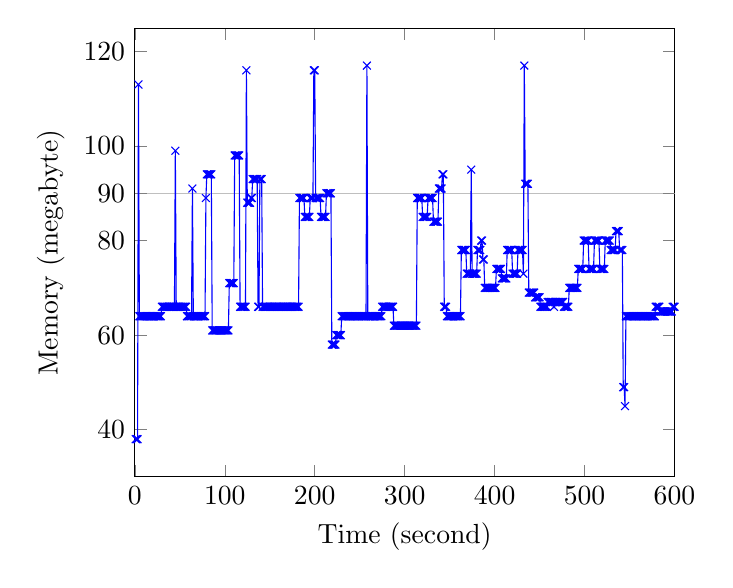
\begin{tikzpicture}
	\begin{axis}[
		xlabel=Time (second),
		xmin=0, xmax=600,
		extra y ticks={90},
		extra tick style={grid=major},
%		ymin=45000, ymax=160000,
%       scaled ticks=false,
%yticklabel style={
%        /pgf/number format/precision=0,
%        /pgf/number format/fixed
%},
		ylabel=Memory (megabyte),
%    legend style={
%        cells={anchor=east},
%        legend pos=outer north east,
%    }
]
	\addplot[color=blue,mark=x] coordinates {
(1   ,38)
(2   ,38)
(3   ,38)
(4   ,113)
(5   ,64)
(6   ,64)
(7   ,64)
(8   ,64)
(9   ,64)
(10  ,64)
(11  ,64)
(12  ,64)
(13  ,64)
(14  ,64)
(15  ,64)
(16  ,64)
(17  ,64)
(18  ,64)
(19  ,64)
(20  ,64)
(21  ,64)
(22  ,64)
(23  ,64)
(24  ,64)
(25  ,64)
(26  ,64)
(27  ,64)
(28  ,64)
(29  ,64)
(30  ,66)
(31  ,66)
(32  ,66)
(33  ,66)
(34  ,66)
(35  ,66)
(36  ,66)
(37  ,66)
(38  ,66)
(39  ,66)
(40  ,66)
(41  ,66)
(42  ,66)
(43  ,66)
(44  ,66)
(45  ,99)
(46  ,66)
(47  ,66)
(48  ,66)
(49  ,66)
(50  ,66)
(51  ,66)
(52  ,66)
(53  ,66)
(54  ,66)
(55  ,66)
(56  ,66)
(57  ,66)
(58  ,64)
(59  ,64)
(60  ,64)
(61  ,64)
(62  ,64)
(63  ,64)
(64  ,91)
(65  ,64)
(66  ,64)
(67  ,64)
(68  ,64)
(69  ,64)
(70  ,64)
(71  ,64)
(72  ,64)
(73  ,64)
(74  ,64)
(75  ,64)
(76  ,64)
(77  ,64)
(78  ,64)
(79  ,89)
(80  ,94)
(81  ,94)
(82  ,94)
(83  ,94)
(84  ,94)
(85  ,94)
(86  ,61)
(87  ,61)
(88  ,61)
(89  ,61)
(90  ,61)
(91  ,61)
(92  ,61)
(93  ,61)
(94  ,61)
(95  ,61)
(96  ,61)
(97  ,61)
(98  ,61)
(99  ,61)
(100 ,61)
(101 ,61)
(102 ,61)
(103 ,61)
(104 ,61)
(105 ,71)
(106 ,71)
(107 ,71)
(108 ,71)
(109 ,71)
(110 ,71)
(111 ,98)
(112 ,98)
(113 ,98)
(114 ,98)
(115 ,98)
(116 ,98)
(117 ,66)
(118 ,66)
(119 ,66)
(120 ,66)
(121 ,66)
(122 ,66)
(123 ,66)
(124 ,116)
(125 ,88)
(126 ,88)
(127 ,88)
(128 ,88)
(129 ,89)
(130 ,89)
(131 ,93)
(132 ,93)
(133 ,93)
(134 ,93)
(135 ,93)
(136 ,93)
(137 ,66)
(138 ,66)
(139 ,93)
(140 ,93)
(141 ,93)
(142 ,66)
(143 ,66)
(144 ,66)
(145 ,66)
(146 ,66)
(147 ,66)
(148 ,66)
(149 ,66)
(150 ,66)
(151 ,66)
(152 ,66)
(153 ,66)
(154 ,66)
(155 ,66)
(156 ,66)
(157 ,66)
(158 ,66)
(159 ,66)
(160 ,66)
(161 ,66)
(162 ,66)
(163 ,66)
(164 ,66)
(165 ,66)
(166 ,66)
(167 ,66)
(168 ,66)
(169 ,66)
(170 ,66)
(171 ,66)
(172 ,66)
(173 ,66)
(174 ,66)
(175 ,66)
(176 ,66)
(177 ,66)
(178 ,66)
(179 ,66)
(180 ,66)
(181 ,66)
(182 ,66)
(183 ,89)
(184 ,89)
(185 ,89)
(186 ,89)
(187 ,89)
(188 ,89)
(189 ,85)
(190 ,85)
(191 ,85)
(192 ,85)
(193 ,85)
(194 ,85)
(195 ,89)
(196 ,89)
(197 ,89)
(198 ,89)
(199 ,116)
(200 ,116)
(201 ,89)
(202 ,89)
(203 ,89)
(204 ,89)
(205 ,89)
(206 ,89)
(207 ,85)
(208 ,85)
(209 ,85)
(210 ,85)
(211 ,85)
(212 ,85)
(213 ,90)
(214 ,90)
(215 ,90)
(216 ,90)
(217 ,90)
(218 ,90)
(219 ,58)
(220 ,58)
(221 ,58)
(222 ,58)
(223 ,58)
(224 ,60)
(225 ,60)
(226 ,60)
(227 ,60)
(228 ,60)
(229 ,60)
(230 ,64)
(231 ,64)
(232 ,64)
(233 ,64)
(234 ,64)
(235 ,64)
(236 ,64)
(237 ,64)
(238 ,64)
(239 ,64)
(240 ,64)
(241 ,64)
(242 ,64)
(243 ,64)
(244 ,64)
(245 ,64)
(246 ,64)
(247 ,64)
(248 ,64)
(249 ,64)
(250 ,64)
(251 ,64)
(252 ,64)
(253 ,64)
(254 ,64)
(255 ,64)
(256 ,64)
(257 ,64)
(258 ,117)
(259 ,64)
(260 ,64)
(261 ,64)
(262 ,64)
(263 ,64)
(264 ,64)
(265 ,64)
(266 ,64)
(267 ,64)
(268 ,64)
(269 ,64)
(270 ,64)
(271 ,64)
(272 ,64)
(273 ,64)
(274 ,64)
(275 ,66)
(276 ,66)
(277 ,66)
(278 ,66)
(279 ,66)
(280 ,66)
(281 ,66)
(282 ,66)
(283 ,66)
(284 ,66)
(285 ,66)
(286 ,66)
(287 ,66)
(288 ,62)
(289 ,62)
(290 ,62)
(291 ,62)
(292 ,62)
(293 ,62)
(294 ,62)
(295 ,62)
(296 ,62)
(297 ,62)
(298 ,62)
(299 ,62)
(300 ,62)
(301 ,62)
(302 ,62)
(303 ,62)
(304 ,62)
(305 ,62)
(306 ,62)
(307 ,62)
(308 ,62)
(309 ,62)
(310 ,62)
(311 ,62)
(312 ,62)
(313 ,62)
(314 ,89)
(315 ,89)
(316 ,89)
(317 ,89)
(318 ,89)
(319 ,89)
(320 ,85)
(321 ,85)
(322 ,85)
(323 ,85)
(324 ,85)
(325 ,85)
(326 ,89)
(327 ,89)
(328 ,89)
(329 ,89)
(330 ,89)
(331 ,89)
(332 ,84)
(333 ,84)
(334 ,84)
(335 ,84)
(336 ,84)
(337 ,84)
(338 ,91)
(339 ,91)
(340 ,91)
(341 ,91)
(342 ,94)
(343 ,94)
(344 ,66)
(345 ,66)
(346 ,66)
(347 ,64)
(348 ,64)
(349 ,64)
(350 ,64)
(351 ,64)
(352 ,64)
(353 ,64)
(354 ,64)
(355 ,64)
(356 ,64)
(357 ,64)
(358 ,64)
(359 ,64)
(360 ,64)
(361 ,64)
(362 ,64)
(363 ,78)
(364 ,78)
(365 ,78)
(366 ,78)
(367 ,78)
(368 ,78)
(369 ,73)
(370 ,73)
(371 ,73)
(372 ,73)
(373 ,73)
(374 ,95)
(375 ,73)
(376 ,73)
(377 ,73)
(378 ,73)
(379 ,73)
(380 ,73)
(381 ,78)
(382 ,78)
(383 ,78)
(384 ,78)
(385 ,80)
(386 ,80)
(387 ,76)
(388 ,76)
(389 ,70)
(390 ,70)
(391 ,70)
(392 ,70)
(393 ,70)
(394 ,70)
(395 ,70)
(396 ,70)
(397 ,70)
(398 ,70)
(399 ,70)
(400 ,70)
(401 ,70)
(402 ,74)
(403 ,74)
(404 ,74)
(405 ,74)
(406 ,74)
(407 ,74)
(408 ,72)
(409 ,72)
(410 ,72)
(411 ,72)
(412 ,72)
(413 ,72)
(414 ,78)
(415 ,78)
(416 ,78)
(417 ,78)
(418 ,78)
(419 ,78)
(420 ,73)
(421 ,73)
(422 ,73)
(423 ,73)
(424 ,73)
(425 ,73)
(426 ,78)
(427 ,78)
(428 ,78)
(429 ,78)
(430 ,78)
(431 ,78)
(432 ,73)
(433 ,117)
(434 ,92)
(435 ,92)
(436 ,92)
(437 ,92)
(438 ,69)
(439 ,69)
(440 ,69)
(441 ,69)
(442 ,69)
(443 ,69)
(444 ,69)
(445 ,68)
(446 ,68)
(447 ,68)
(448 ,68)
(449 ,68)
(450 ,68)
(451 ,66)
(452 ,66)
(453 ,66)
(454 ,66)
(455 ,66)
(456 ,66)
(457 ,66)
(458 ,66)
(459 ,67)
(460 ,67)
(461 ,67)
(462 ,67)
(463 ,67)
(464 ,67)
(465 ,67)
(466 ,66)
(467 ,67)
(468 ,67)
(469 ,67)
(470 ,67)
(471 ,67)
(472 ,67)
(473 ,67)
(474 ,67)
(475 ,67)
(476 ,67)
(477 ,66)
(478 ,66)
(479 ,66)
(480 ,66)
(481 ,66)
(482 ,66)
(483 ,70)
(484 ,70)
(485 ,70)
(486 ,70)
(487 ,70)
(488 ,70)
(489 ,70)
(490 ,70)
(491 ,70)
(492 ,70)
(493 ,74)
(494 ,74)
(495 ,74)
(496 ,74)
(497 ,74)
(498 ,74)
(499 ,80)
(500 ,80)
(501 ,80)
(502 ,80)
(503 ,80)
(504 ,80)
(505 ,74)
(506 ,74)
(507 ,74)
(508 ,74)
(509 ,74)
(510 ,74)
(511 ,80)
(512 ,80)
(513 ,80)
(514 ,80)
(515 ,80)
(516 ,80)
(517 ,74)
(518 ,74)
(519 ,74)
(520 ,74)
(521 ,74)
(522 ,74)
(523 ,80)
(524 ,80)
(525 ,80)
(526 ,80)
(527 ,80)
(528 ,80)
(529 ,78)
(530 ,78)
(531 ,78)
(532 ,78)
(533 ,78)
(534 ,78)
(535 ,82)
(536 ,82)
(537 ,82)
(538 ,82)
(539 ,78)
(540 ,78)
(541 ,78)
(542 ,78)
(543 ,49)
(544 ,49)
(545 ,45)
(546 ,64)
(547 ,64)
(548 ,64)
(549 ,64)
(550 ,64)
(551 ,64)
(552 ,64)
(553 ,64)
(554 ,64)
(555 ,64)
(556 ,64)
(557 ,64)
(558 ,64)
(559 ,64)
(560 ,64)
(561 ,64)
(562 ,64)
(563 ,64)
(564 ,64)
(565 ,64)
(566 ,64)
(567 ,64)
(568 ,64)
(569 ,64)
(570 ,64)
(571 ,64)
(572 ,64)
(573 ,64)
(574 ,64)
(575 ,64)
(576 ,64)
(577 ,64)
(578 ,64)
(579 ,66)
(580 ,66)
(581 ,66)
(582 ,66)
(583 ,66)
(584 ,65)
(585 ,65)
(586 ,65)
(587 ,65)
(588 ,65)
(589 ,65)
(590 ,65)
(591 ,65)
(592 ,65)
(593 ,65)
(594 ,65)
(595 ,65)
(596 ,65)
(597 ,65)
(598 ,66)
(599 ,66)
(600 ,66)
	};
	\end{axis}
\end{tikzpicture}
}
\caption{Memory usage over time of the embedded device controller with Lesser Evil.}
\label{fig:graph}
\end{figure}


Based on the logs written by Lesser Evil, there were several actions executed. Both the $\mathit{trigger\_gc}$ and the $\mathit{terminate\_proc}$ actions were invoked by Lesser Evil. Actions were triggered frequently but the cool down period was always respected. As there were processes terminated by Lesser Evil, we need to confirm that the right processes were selected for termination. As only L-sized requests failed in both experiments (9 and 8 errors), we conclude that Lesser Evil chose the right processes to terminate, did not interfere with the rest of the processes, and effectively controlled the memory usage of the SUT, confirming Hypothesis \#3. Due to the failed requests there was a temporary, partial system degradation that effected only the requesters of L-sized requests. However, a temporary, partial system degradation is still a better choice compared to the test runs where the SUT got terminated by the Linux OOM manager and, therefore, a major outage occurred. The experiments confirm Hypothesis \#2.

\paragraph{Overhead}
We started the SUT with and without Lesser Evil and recorded the rss size~\cite{ps} for a minute. Then, we calculated the difference point by point of the recorded values; the difference we got is the memory used by the Lesser Evil agent code. The minimum, median and maximum values of memory used by the agent code are: 848~KB, 1~000~KB, 1~148~KB, which  we consider low enough. The experiment confirms  Hypothesis \#4.

\subsection{Conclusion \& Limitations}
\label{limitations}
%In this section we draw conclusions and discuss the current limitations of Lesser Evil.

The experiments confirm all 4 hypotheses. Lesser Evil can control the memory usage of an Erlang node and avoid major outage. Its negative impact on the overall system is minimal. Considering the embedded device controller use case, which is the primary use case of Lesser Evil, that includes an Erlang system with high availability but with very limited memory and slow processing capabilities, Lesser Evil can help in scenarios where a few unusually large requests arrive that take long to process and fill up the available memory. %Considering the other use case that include an Erlang system with high availability, large amount of memory and fast processing capabilities, Lesser Evil may have negative impact on the tail latencies, nonetheless, can help in cases with ever growing memory usage, and can offer limited help when an unplanned, large load appears on the system.

We have experimented with other use cases. We have found that if the memory pressure is due to a continuously arriving, vast amount of short lived (ca 2 milliseconds) processes with high memory consumption, Lesser Evil cannot effectively control the memory usage of the Erlang node. 
To fix memory pressure, Lesser Evil would need to execute the $terminate\_proc$ action without respecting the cool down internal: risking to cause the termination of the Erlang node.
%The reason why Lesser Evil cannot effectively help is due to the cool down interval. To have effect in such situations, Lesser Evil would need to execute 
%the $terminate\_proc$ action as often as possible but that could cause the termination of the whole Erlang node.

\subsection{Threats to Validity}
Our evaluation is subject to threats to validity. The results were obtained from an Erlang system, and hence, they cannot necessarily be generalized to all Erlang systems. We minimised this threat in three ways. First, by reviewing the most widespread use cases of Erlang to  build a representative test system that characterises well the given use case of Erlang.  Second, by building the test subject using Erlang applications (cowboy, ranch, etc.) that are widespread and heavily used in real-life Erlang applications, and are not built by the authors. Third, by ensuring that the code written by the authors is very small (202 lines out of 267K lines) considering the size of the project, and Lesser Evil monitors an application (\verb+ranch+~\cite{ranch}) that is independent from the authors.

\section{Related Work}
Memory pressure has always been an important challenge of the research and practitioner community. The topic has been discussed in different contexts ranging from operating systems to software libraries targeting specific software applications.

Considering operating system level, there is a generic solution for Linux systems, called the OOM manager~\cite{oom}.  The OOM manager is tasked to monitor the host and, under low memory conditions, select and terminate an OS process to treat memory pressure. Its goal is to protect the availability of the overall host. It employs a strategy to select new, non-user preferred processes that have high memory usage. Considering Erlang systems, our experience and the evaluation presented in this paper show that OOM is not a help, we have never seen a case when killing the Erlang node solved the underlying problem. Instead, it damaged the Erlang systems. Lesser Evil and the OOM Manager work on different abstraction level, however, both protect the overall system availability, employ a strategy and treat memory pressure by killing processes.

Virtualisation techniques have become significant to better utilise available resources and to isolate applications. An example is Apache Mesos~\cite{embracingfailures,mesos2} that sits between the application layer and the operating system and makes it easier to deploy and manage applications in large-scale clustered environments more efficiently. Apache Mesos supports oversubscription~\cite{mesos-oversub} for better resource utilisation with the promise of keeping QoS metrics. Their approach is to monitor the entire host and if CPU pressure occurs the QoS controller kills revocable tasks. To further improve killing tasks when oversubscription occurs, the authors of \cite{UAkiller} propose a user-assisted OOM killer in kernel space for agile task killing. Lesser Evil and the Mesos's QoS controller have different focus (memory versus CPU), however, both select and terminate entities that are non-critical to the system. 

As there is no general solution for programming language and runtime level, researchers have proposed various solutions to better manage specific use cases~\cite{app5,app7,app6,itasks}. Browsing through the articles, one can notice that there has been a targeted interest in Java programs. ITask proposed in \cite{itasks} is a promising choice for Java workflow applications that requires code modification, however, promises protection of tasks and performance improvements in high load scenarios. This is a considerable benefit compared to Lesser Evil, however, on the other hand rewriting applications is not required by Lesser Evil. Besides, as Erlang applications often employs restart strategies for important worker processes offering the restoration of interrupted tasks, it is not a necessity. The authors of \cite{hedgetechnique} proposed a more general solution for handling out of memory errors in Java applications. The idea is to overallocate memory that is not used and release the non-used memory when out of memory errors occur. The authors of \cite{yang2006cramm} looks at the problem from another perspective, taming the garbage collection, and proposes a system that enables garbage-collected applications to predict an appropriate heap size, allowing the system to maintain high performance while adjusting dynamically to changing memory pressure.

When embedded systems are targeted, memory management becomes more  critical as memory is more limited and virtual memory is often disabled. Researchers have proposed several low level memory management techniques that focus on memory allocation strategies and minimises memory fragmentation~\cite{embedded-low1,embedded-low3}. The authors of \cite{embedded3} observed that application performance is impacted by the employed memory allocation strategy in embedded systems. They propose to manage memory per task and introduce a runtime scheduler for memory management policy switching and kernel overlapping. Their evaluation suggests that their approach can treat memory pressure and improve response time. Virtualisation ensures isolation of applications that is necessary in smart consumer electronics. However, with a  virtualised embedded device, flexible memory management is required to run multiple VMs efficiently on resource-constrained hardware. The authors of \cite{embedded4} tackle the challenge by introducing an in-memory compressed swap device (CSW) that prioritises the memory reservations of the critical applications running on the embedded device by swapping out only the memory of third-party applications in response to memory pressure. Lesser Evil and CSW employ different compensating actions but both activate when low memory conditions occur and distinguish between critical and non-critical entities.

\section{Conclusion}
In this paper we have proposed and implemented an approach, called Lesser Evil, that can treat low memory pressure in Erlang systems without the need of any code modification. Lesser Evil embraces failures to protect overall system availability. It monitors the running program and upon low memory conditions selects some non-critical entities based on the badness metric and execute compensating actions on the selected entities to help the system avoid a major outage. Lesser Evil is ready to use and is applicable to any Erlang systems. The prototype implementation is available on GitHub~\cite{lesser-evil}.
%The evaluation supports that an embedded Erlang system can avoid a major outage and keep functioning under low memory conditions with the help of our approach. %The evaluation also shows that Lesser Evil can offer limited help for large scale Erlang deployments.

The evaluation shows that Lesser Evil can control the memory usage of an Erlang node and an embedded Erlang system can avoid a major outage and keep functioning under low memory conditions with the help of our approach. We have confirmed that Lesser Evil's negative impact on the overall system is minimal, and Lesser Evil's strategy is correct: it is able to identify and execute compensating actions on the components most responsible for the situation without damaging the other components or the overall system.

%\newpage
%Considering future work, we plan to research more programming languages to see if Lesser Evil is applicable, and to further evaluate Lesser Evil on industrial applications and present our results. Researching a strategy to help CPU-bound applications is on the horizon. Besides, as Lesser Evil knows the current memory conditions, the agent code can be extended to provide recommendation to applications whether they can increase the level of concurrency.

%
% ---- Bibliography ----
%
% BibTeX users should specify bibliography style 'splncs04'.
% References will then be sorted and formatted in the correct style.
%
 \bibliographystyle{splncs04}
 \bibliography{bibliography}
 
\end{document}
